%! TEX root = ../aminhash.tex

\section{Conclusion}

We have shown that it is possible to substantially improve upon the traditional MinHash estimator in the one-way setting.

\begin{figure}[h]
   \centering
   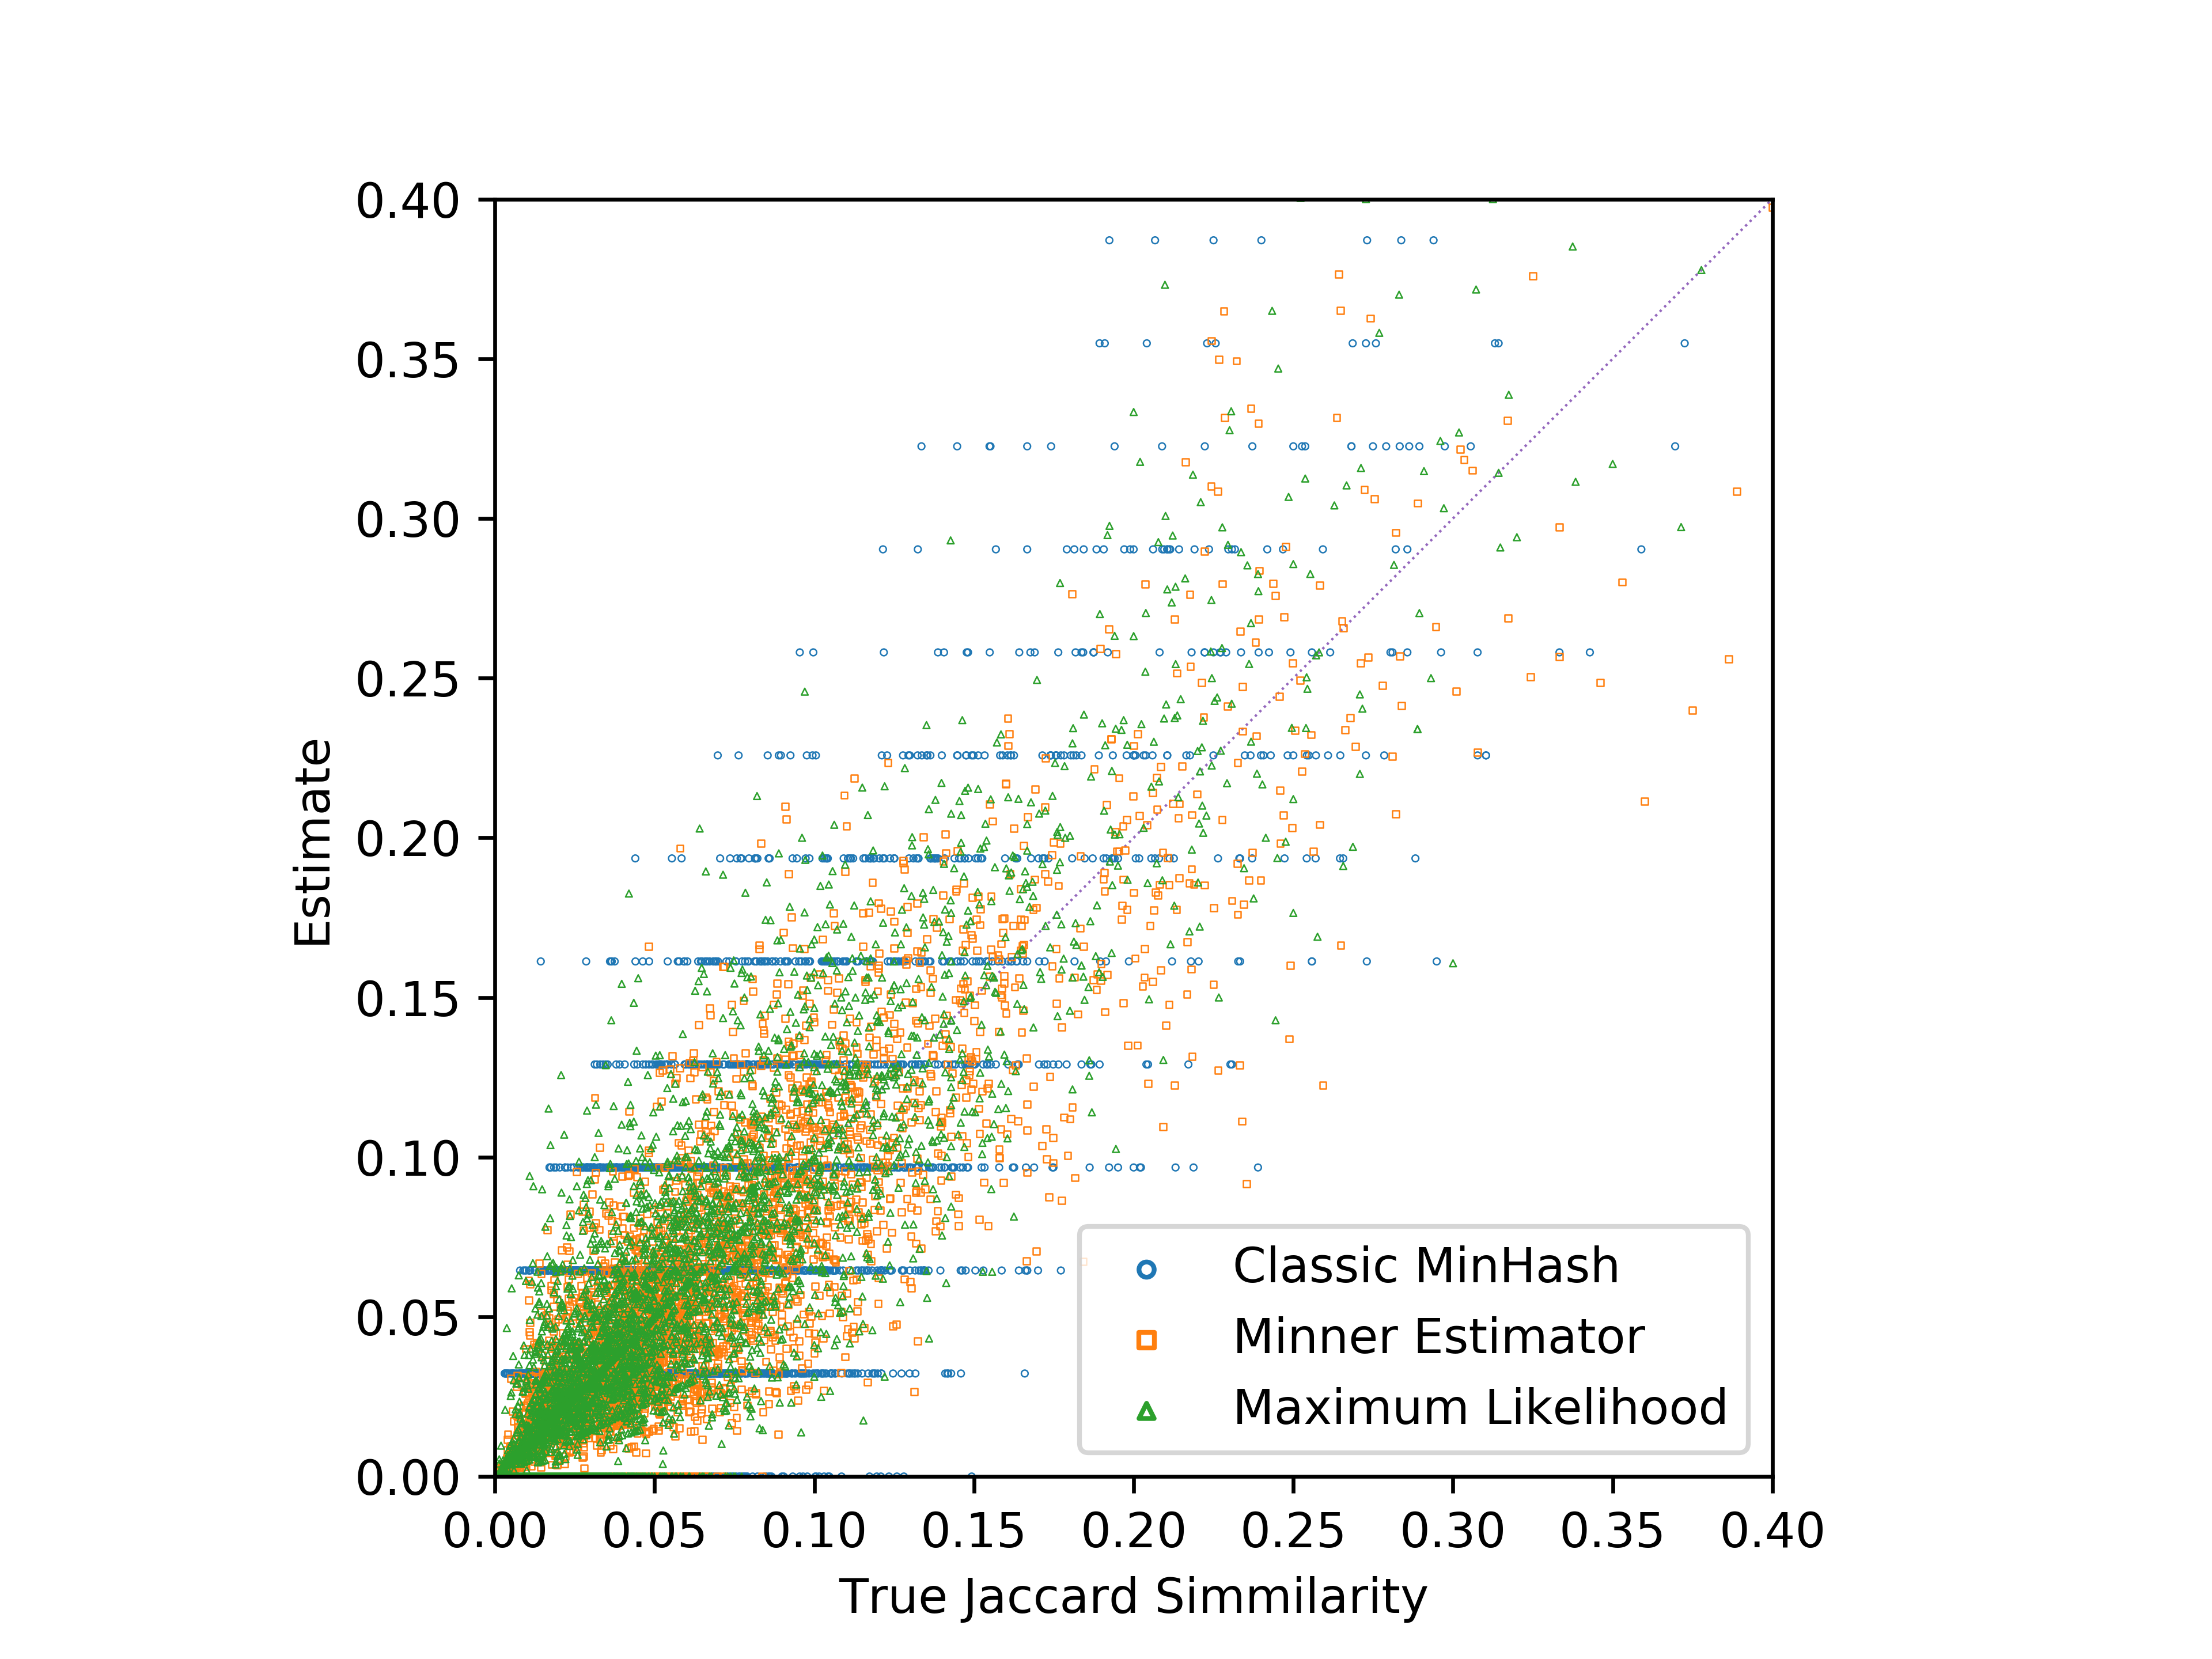
\includegraphics[trim=10 0 10 30,clip,width=\linewidth]{figures/scatter}
   \caption{Typical query in the Netflix dataset with 5,000 pairs, using $K=31$.
      The Classical Estimator shows clear banding, due to it taking only $K$ different values.
   }
\end{figure}


\section{Open Problems}

Can we also better estimate other types of MinHash?
\begin{enumerate}
   \item Weighted MinHash
   \item $b$-bit MinHash
   \item Bottom-$k$ MinHash
   \item Find the best sketch for sets in general. Like how Supermajorities is best for queries.
   \item Use a prior better than uniform for $Y$.
      One might for example take into account skew distributions, where some tokens are more likely than other.
\end{enumerate}


